\documentclass[dvipdfmx,a4paper,12pt]{jsarticle}
\usepackage[margin=21mm]{geometry}
\usepackage{graphicx}
\usepackage{amsmath,amssymb}
\usepackage{enumitem}
\usepackage{tikz}
\usepackage{float}

\usetikzlibrary{arrows.meta,calc,patterns,positioning}

\setlength{\parindent}{0pt}
\setlength{\parskip}{0.35em}
\setlist[itemize]{leftmargin=2em,itemsep=0.2em,topsep=0.3em}
\setlist[enumerate]{leftmargin=2em,itemsep=0.4em,topsep=0.3em}

\newcommand{\chap}[1]{\vspace{1.0em}{\Large #1}\par\vspace{0.25em}\hrule\vspace{0.55em}}
\newcommand{\subchap}[1]{\vspace{0.7em}{\large #1}\par\vspace{0.15em}}
\newcommand{\smallcaptext}[1]{\begin{center}\small #1\end{center}}
\newcommand{\keybox}[1]{\begin{center}\fbox{\begin{minipage}{0.94\linewidth}#1\end{minipage}}\end{center}}

\begin{document}

\begin{center}
{\LARGE 数学1A 第8回レジュメ}\\[0.4em]
多変数関数・偏微分・可微分性
\end{center}

\chap{授業のねらい}

この回では，一変数関数の微分を二変数関数へ広げる。特に，
\begin{itemize}
\item 多変数関数の定義域，グラフ，等高線を図で理解すること，
\item 偏微分を「一つの方向だけの変化率」として理解すること，
\item 偏微分可能性と可微分性の違いを区別すること，
\item $C^n$ 級関数と混合偏微分の意味を理解すること
\end{itemize}
を目標とする。

\begin{center}
\begin{tikzpicture}[>=Latex,x=1cm,y=1cm]
\draw[rounded corners=4pt,draw=blue!55!black,fill=blue!5] (-4.8,-1.3) rectangle (-2.2,1.3);
\node at (-3.5,0.55) {$\mathbb R^2$};
\node at (-3.5,0.05) {入力};
\node at (-3.5,-0.55) {$(x,y)$};
\draw[->,thick] (-2.05,0) -- (-0.65,0);
\node[above] at (-1.35,0) {$f$};
\draw[rounded corners=4pt,draw=teal!55!black,fill=teal!5] (-0.45,-1.3) rectangle (2.15,1.3);
\node at (0.85,0.55) {$\mathbb R$};
\node at (0.85,0.05) {出力};
\node at (0.85,-0.55) {$z=f(x,y)$};
\draw[->,thick] (2.35,0) -- (3.75,0);
\node[draw=orange!65!black,fill=orange!10,rounded corners=4pt,minimum width=2.1cm,minimum height=1.4cm] at (5.0,0) {曲面・等高線};
\end{tikzpicture}
\smallcaptext{二変数関数は，平面上の点 $(x,y)$ に数 $z$ を対応させる。}
\end{center}

\chap{1. 多変数関数}

\subchap{1.1 定義}

2つ以上の変数をもつ関数を多変数関数という。

\begin{itemize}
\item 2変数関数は $z=f(x,y)$ と書く。
\item 3変数関数は $w=f(x,y,z)$ と書く。
\end{itemize}

工学では，温度，圧力，電位，速度場などが多変数関数として現れる。たとえば金属板の温度は，位置 $(x,y)$ によって値が変わるので $T(x,y)$ と表せる。

\subchap{1.2 定義域}

関数が意味をもつ入力全体を定義域という。二変数関数では，定義域は平面内の領域として表されることが多い。

\begin{itemize}
\item 分母が $0$ にならない範囲を考える。
\item ルートの中が $0$ 以上になる範囲を考える。
\item 対数の中が正になる範囲を考える。
\end{itemize}

\begin{center}
\begin{minipage}{0.48\linewidth}
\centering
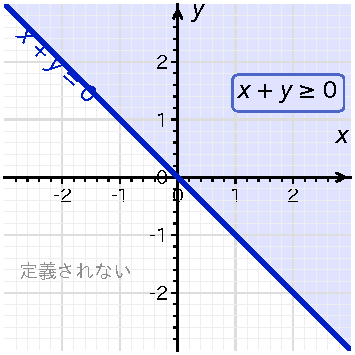
\includegraphics[width=0.92\linewidth]{figures/domain_sqrt.pdf}
\smallcaptext{$f(x,y)=\sqrt{x+y}$ の定義域}
\end{minipage}
\hfill
\begin{minipage}{0.48\linewidth}
\centering
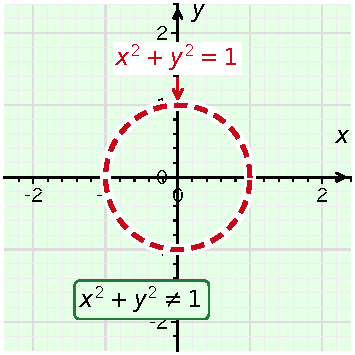
\includegraphics[width=0.92\linewidth]{figures/domain_rational.pdf}
\smallcaptext{$f(x,y)=\dfrac{1}{x^2+y^2-1}$ の定義域}
\end{minipage}
\end{center}

\subchap{1.3 グラフと等高線}

2変数関数 $z=f(x,y)$ のグラフは空間内の曲面になる。また，定数 $c$ に対して
$$
f(x,y)=c
$$
を満たす点の集合を等高線という。等高線は，曲面を水平な平面 $z=c$ で切ったときの影を $xy$ 平面に描いたものである。

\begin{center}
\begin{minipage}{0.48\linewidth}
\centering
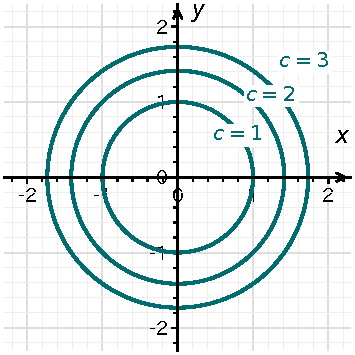
\includegraphics[width=0.92\linewidth]{figures/paraboloid_contours.pdf}
\smallcaptext{$f(x,y)=x^2+y^2$ の等高線}
\end{minipage}
\hfill
\begin{minipage}{0.48\linewidth}
\centering
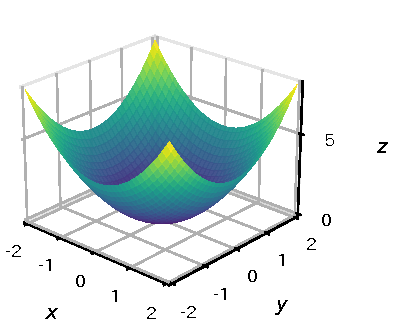
\includegraphics[width=0.95\linewidth]{figures/paraboloid_surface.pdf}
\smallcaptext{$z=x^2+y^2$ のグラフ}
\end{minipage}
\end{center}

\begin{center}
\begin{minipage}{0.48\linewidth}
\centering
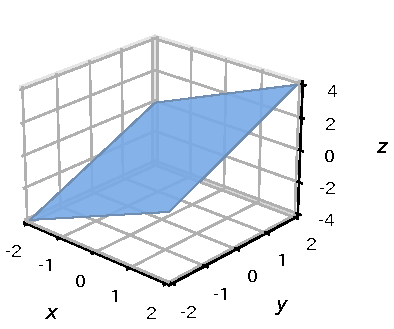
\includegraphics[width=0.95\linewidth]{figures/plane_surface.pdf}
\smallcaptext{$z=x+y$ は平面である。}
\end{minipage}
\hfill
\begin{minipage}{0.48\linewidth}
\centering
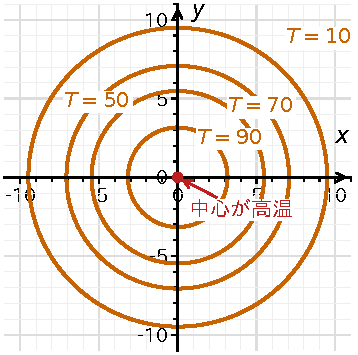
\includegraphics[width=0.92\linewidth]{figures/temperature_contours.pdf}
\smallcaptext{$T(x,y)=100-x^2-y^2$ の等温線}
\end{minipage}
\end{center}

\subchap{例題}

\begin{enumerate}
\item 次の関数の等高線を考えよ。$f(x,y)=x^2+y^2$
\item 次の関数のグラフの形を説明せよ。$f(x,y)=x+y$
\item 次の関数の等高線を考えよ。$f(x,y)=x-y$
\item 次の関数の等高線を考え，中心から離れると値がどう変化するか説明せよ。$f(x,y)=4-x^2-y^2$
\item 工学的な量として，温度分布 $T(x,y)=100-x^2-y^2$ を考える。この関数の意味を説明せよ。
\end{enumerate}

\chap{2. 偏微分の定義}

\subchap{2.1 偏微分とは}

多変数関数で，ある1つの変数だけを変化させ，他の変数を固定して微分することを偏微分という。

2変数関数 $f(x,y)$ に対して，$\dfrac{\partial f}{\partial x}$ は $y$ を定数とみなして $x$ で微分したもの，$\dfrac{\partial f}{\partial y}$ は $x$ を定数とみなして $y$ で微分したものである。

\begin{center}
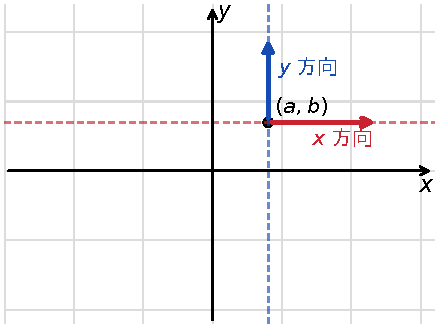
\includegraphics[width=0.48\linewidth]{figures/partial_directions.pdf}
\smallcaptext{偏微分では，一方の方向だけに動かして変化率を見る。}
\end{center}

\subchap{2.2 定義}

点 $(a,b)$ における $x$ に関する偏微分係数は
$$
f_x(a,b)
=
\lim_{h\to 0}
\frac{f(a+h,b)-f(a,b)}{h}
$$
で定義される。同様に，$y$ に関する偏微分係数は
$$
f_y(a,b)
=
\lim_{h\to 0}
\frac{f(a,b+h)-f(a,b)}{h}
$$
で定義される。

\subchap{2.3 記号}

偏導関数は
$$
f_x,\quad f_y,\quad \frac{\partial f}{\partial x},\quad \frac{\partial f}{\partial y}
$$
などと書く。文脈によっては $f_x(x,y)$，$f_y(x,y)$ のように変数を明記する。

\subchap{2.4 幾何学的意味}

$\dfrac{\partial f}{\partial x}$ は $x$ 方向の変化率，$\dfrac{\partial f}{\partial y}$ は $y$ 方向の変化率を表す。曲面 $z=f(x,y)$ を $y=b$ で切ると一変数関数 $z=f(x,b)$ が得られ，その傾きが $f_x(a,b)$ である。

\begin{center}
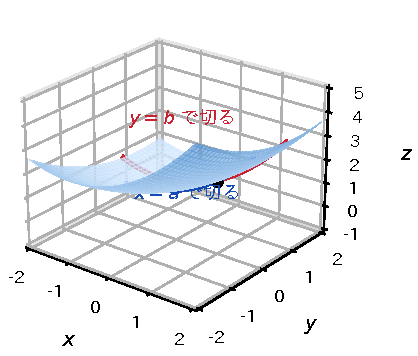
\includegraphics[width=0.70\linewidth]{figures/partial_surface.pdf}
\smallcaptext{赤い曲線の傾きが $x$ 方向の偏微分，青い曲線の傾きが $y$ 方向の偏微分を表す。}
\end{center}

\subchap{例題}

\begin{enumerate}
\item 次の関数の $x$ に関する偏微分を求めよ。$f(x,y)=x^2+3xy+y^2$
\item 次の関数の $y$ に関する偏微分を求めよ。$f(x,y)=x^2\sin y$
\item 次の関数の偏導関数 $f_x,\ f_y$ を求めよ。$f(x,y)=e^{xy}$
\item 次の関数の偏導関数を求めよ。$f(x,y,z)=x^2y+yz^3$
\item 温度分布 $T(x,y)=50+2x-y^2$ について，$\partial T/\partial x$，$\partial T/\partial y$ の意味を説明せよ。
\end{enumerate}

\chap{3. 偏微分可能性と可微分性}

\subchap{3.1 偏微分可能}

点 $(a,b)$ において $f_x(a,b)$，$f_y(a,b)$ が存在するとき，その点で偏微分可能という。ただし，偏微分可能であっても，必ずしも関数が滑らかとは限らない。

\subchap{3.2 可微分}

関数 $f(x,y)$ が点 $(a,b)$ の近くで一次式によりよく近似できるとき，その点で可微分という。可微分であれば，
$$
f(a+\Delta x,b+\Delta y)
$$
は
$$
f(a,b)+f_x(a,b)\Delta x+f_y(a,b)\Delta y
$$
で近似できる。

\begin{center}
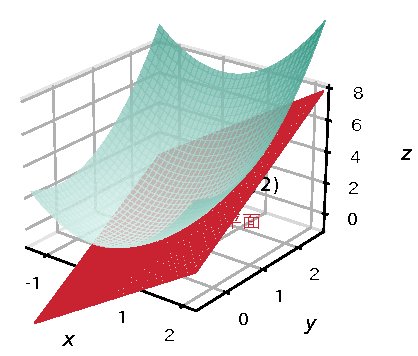
\includegraphics[width=0.70\linewidth]{figures/tangent_plane.pdf}
\smallcaptext{$z=x^2+y^2$ を点 $(1,1,2)$ の近くで平面 $z=2x+2y-2$ によって近似する。}
\end{center}

\subchap{3.3 全微分}

可微分な関数に対して
$$
df=f_xdx+f_ydy
$$
を全微分という。小さい変化に対して
$$
\Delta f\simeq f_x\Delta x+f_y\Delta y
$$
と考えることができる。

\subchap{3.4 接平面}

$z=f(x,y)$ が可微分なら，点 $(a,b,f(a,b))$ における接平面は
$$
z=f(a,b)+f_x(a,b)(x-a)+f_y(a,b)(y-b)
$$
で表される。

\keybox{接平面は，曲面を点の近くで一次式に置き換えたものである。これは一変数関数でいう接線の二変数版である。}

\subchap{3.5 重要な十分条件}

$f_x$，$f_y$ が点の近くで存在し，かつ連続ならば，$f$ はその点で可微分である。つまり，偏導関数が連続なら可微分性が保証される。

\begin{center}
\begin{tikzpicture}[>=Latex,node distance=1.5cm]
\node[draw=blue!60!black,fill=blue!5,rounded corners=3pt,minimum width=4.3cm,minimum height=0.9cm] (a) {$f_x,\ f_y$ が近くで連続};
\node[draw=teal!65!black,fill=teal!5,rounded corners=3pt,minimum width=3.6cm,minimum height=0.9cm,right=of a] (b) {$f$ は可微分};
\node[draw=orange!75!black,fill=orange!8,rounded corners=3pt,minimum width=3.5cm,minimum height=0.9cm,right=of b] (c) {$f$ は偏微分可能};
\draw[->,thick] (a) -- (b);
\draw[->,thick] (b) -- (c);
\node[below=0.15cm of b] {\small 逆向きは一般には成り立たない};
\end{tikzpicture}
\smallcaptext{連続な偏導関数は可微分性を保証する。}
\end{center}

\subchap{偏微分可能だが可微分でない例}

次の関数は原点で $f_x(0,0)=0$，$f_y(0,0)=0$ をもつが，可微分ではない。
$$
f(x,y)=
\begin{cases}
\dfrac{xy}{\sqrt{x^2+y^2}} & ((x,y)\neq(0,0)),\\[0.7em]
0 & ((x,y)=(0,0)).
\end{cases}
$$
軸方向では値が $0$ になるが，直線 $y=x$ に沿うと $f(x,x)=|x|/\sqrt{2}$ となり，原点付近で一次近似 $0$ だけでは十分に近似できない。

\begin{center}
\begin{minipage}{0.48\linewidth}
\centering
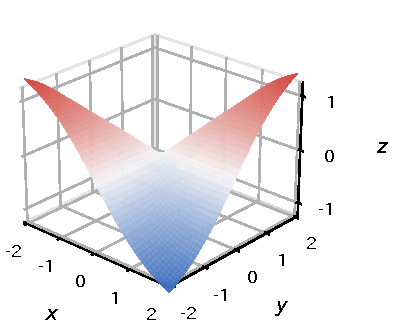
\includegraphics[width=0.95\linewidth]{figures/nondiff_surface.pdf}
\smallcaptext{$xy/\sqrt{x^2+y^2}$ の原点近くの形}
\end{minipage}
\hfill
\begin{minipage}{0.48\linewidth}
\centering
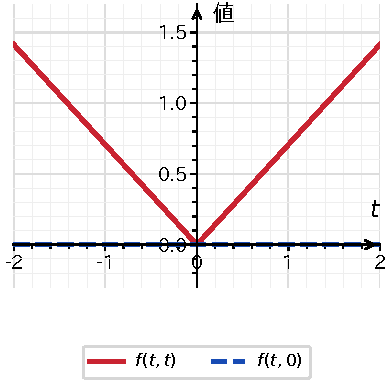
\includegraphics[width=0.95\linewidth]{figures/direction_slice.pdf}
\smallcaptext{軸方向だけを見ると見落とす変化がある。}
\end{minipage}
\end{center}

\subchap{例題}

\begin{enumerate}
\item 次の関数が点 $(1,2)$ で偏微分可能か調べよ。$f(x,y)=x^2+xy+y^2$
\item 次の関数の全微分を求めよ。$f(x,y)=x^2y+y^3$
\item 次の関数の点 $(1,1)$ における接平面を求めよ。$z=x^2+y^2$
\item 次の関数が可微分であるか考えよ。$f(x,y)=|x|+|y|$
\item 次の関数について，偏微分可能性と可微分性の違いを説明せよ。
$$
f(x,y)=
\begin{cases}
\dfrac{xy}{\sqrt{x^2+y^2}} & ((x,y)\neq(0,0)),\\[0.7em]
0 & ((x,y)=(0,0)).
\end{cases}
$$
\end{enumerate}

\chap{4. $C^n$ 級関数}

\subchap{4.1 $C^0$ 級}

関数が連続であるとき，$C^0$ 級という。

\subchap{4.2 $C^1$ 級}

1階偏導関数が存在し，それらが連続であるとき，$C^1$ 級という。二変数関数では，$f_x$，$f_y$ が存在して連続であることを意味する。

\subchap{4.3 $C^2$ 級}

2階偏導関数が存在し，それらが連続であるとき，$C^2$ 級という。2階偏導関数には
$$
f_{xx},\quad f_{xy},\quad f_{yx},\quad f_{yy}
$$
がある。

\subchap{4.4 $C^n$ 級}

$n$ 階までのすべての偏導関数が存在し，連続であるとき，$C^n$ 級という。

\subchap{4.5 $C^\infty$ 級}

すべての階数の偏導関数が存在し，連続であるとき，$C^\infty$ 級という。多項式，指数関数，三角関数を組み合わせた多くの関数は，定義域上で $C^\infty$ 級である。

\begin{center}
\begin{tikzpicture}[>=Latex,node distance=1.25cm]
\node[draw=purple!60!black,fill=purple!6,rounded corners=3pt,minimum width=2.5cm,minimum height=0.9cm] (inf) {$C^\infty$};
\node[draw=blue!60!black,fill=blue!6,rounded corners=3pt,minimum width=2.5cm,minimum height=0.9cm,right=of inf] (c2) {$C^2$};
\node[draw=teal!60!black,fill=teal!6,rounded corners=3pt,minimum width=2.5cm,minimum height=0.9cm,right=of c2] (c1) {$C^1$};
\node[draw=orange!70!black,fill=orange!8,rounded corners=3pt,minimum width=2.5cm,minimum height=0.9cm,right=of c1] (c0) {$C^0$};
\draw[->,thick] (inf) -- (c2);
\draw[->,thick] (c2) -- (c1);
\draw[->,thick] (c1) -- (c0);
\node[below=0.2cm of c2] {\small 右へ行くほど条件が弱い};
\end{tikzpicture}
\smallcaptext{$C^\infty$ 級なら $C^2$ 級，$C^2$ 級なら $C^1$ 級，$C^1$ 級なら $C^0$ 級である。}
\end{center}

\subchap{4.6 混合偏微分}

条件がよければ，
$$
f_{xy}=f_{yx}
$$
が成り立つ。特に $f$ が $C^2$ 級ならば，混合偏微分は等しい。

\begin{center}
\begin{tikzpicture}[>=Latex,x=1cm,y=1cm]
\node[draw=gray!60,fill=gray!7,rounded corners=3pt,minimum width=2.6cm,minimum height=0.8cm] (f) at (0,1.4) {$f$};
\node[draw=red!60!black,fill=red!6,rounded corners=3pt,minimum width=2.6cm,minimum height=0.8cm] (fx) at (-2.4,0) {$f_x$};
\node[draw=blue!60!black,fill=blue!6,rounded corners=3pt,minimum width=2.6cm,minimum height=0.8cm] (fy) at (2.4,0) {$f_y$};
\node[draw=teal!60!black,fill=teal!6,rounded corners=3pt,minimum width=2.6cm,minimum height=0.8cm] (fxy) at (0,-1.5) {$f_{xy}=f_{yx}$};
\draw[->,thick,red!70!black] (f) -- node[left] {$x$ で偏微分} (fx);
\draw[->,thick,blue!70!black] (f) -- node[right] {$y$ で偏微分} (fy);
\draw[->,thick,blue!70!black] (fx) -- node[left] {$y$ で偏微分} (fxy);
\draw[->,thick,red!70!black] (fy) -- node[right] {$x$ で偏微分} (fxy);
\end{tikzpicture}
\smallcaptext{$C^2$ 級では，$x$ で微分してから $y$ で微分しても，順序を入れ替えても同じになる。}
\end{center}

\subchap{$C^n$ 級の見方}

\begin{center}
\begin{minipage}{0.48\linewidth}
\centering
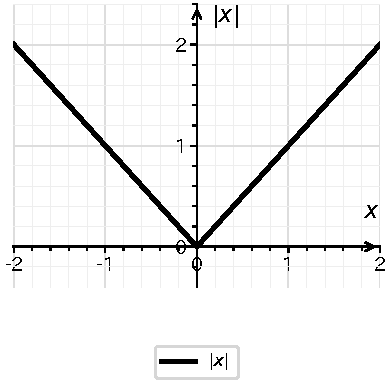
\includegraphics[width=0.95\linewidth]{figures/abs_value.pdf}
\smallcaptext{$|x|$ は $x=0$ で折れている。}
\end{minipage}
\hfill
\begin{minipage}{0.48\linewidth}
\centering
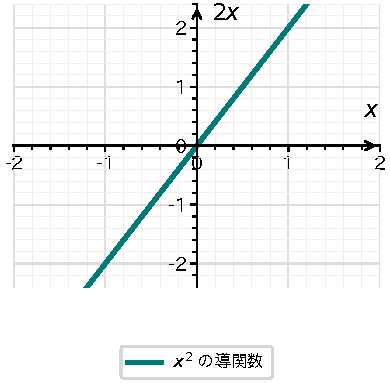
\includegraphics[width=0.95\linewidth]{figures/derivative_line.pdf}
\smallcaptext{$x^2$ はなめらかで，何度でも微分できる。}
\end{minipage}
\end{center}

\subchap{例題}

\begin{enumerate}
\item 次の関数が原点で $C^1$ 級でないことを調べよ。$f(x,y)=|x|+y^2$
\item 次の関数の2階偏導関数を求めよ。$f(x,y)=x^3y+xy^2$
\item 次の関数について，$f_{xy}$ と $f_{yx}$ を求めよ。$f(x,y)=e^{xy}$
\item 次の関数が原点で $C^2$ 級でないことを調べよ。$f(x,y)=x|y|$
\item 次の関数が直線 $x=0$ 上で $C^1$ 級でないことを調べよ。$f(x,y)=|x|+y^2$
\item 次の関数が原点で $C^1$ 級でないことを調べよ。
$$
f(x,y)=
\begin{cases}
\sqrt{x^2+y^2} & ((x,y)\neq(0,0)),\\
0 & ((x,y)=(0,0)).
\end{cases}
$$
\end{enumerate}

\chap{まとめ}

\begin{itemize}
\item 多変数関数は，複数の入力変数をもつ関数である。
\item 偏微分は，1つの変数だけを動かして微分する操作である。
\item 偏微分可能であっても，可微分とは限らない。
\item 偏導関数が連続なら，可微分性が保証される。
\item $C^n$ 級とは，$n$ 階までの偏導関数が連続に存在する関数である。
\item $C^2$ 級なら，$f_{xy}=f_{yx}$ が成り立つ。
\end{itemize}

\end{document}
